\documentclass[12pt, onecolumn]{extarticle}
\usepackage{amsmath}
\usepackage{graphicx}
\usepackage{minted}

\title{System Identification of Non-linear Inverted Pendulum with neural networks}
\author{Jaydeep Nandi, Asim Das, Priyanku Goswami}

\begin{document}
	\maketitle
	\abstract System identification
	
	\section{Introduction} Hi
	\section{Inverted Pendulum System}
	\section{Multi-layer Perceptrons} 
	
	\subsection{\textbf{Introduction}}
	A multi-layer perceptron (MLP) is a class of feed-forward artificial neural network. An MLP consists of at least three layers of nodes. Except for the input nodes, each node is a neuron that uses a nonlinear activation function. MLP utilizes a supervised learning technique called backpropagation for training. Its multiple layers and non-linear activation distinguish MLP from a linear perceptron. It can distinguish data that is not linearly separable. \\ \\  
	The general architecture of a MLP is shown in figure \ref{fig:MLP_1}   
	\begin{figure}[h]
		\centering
		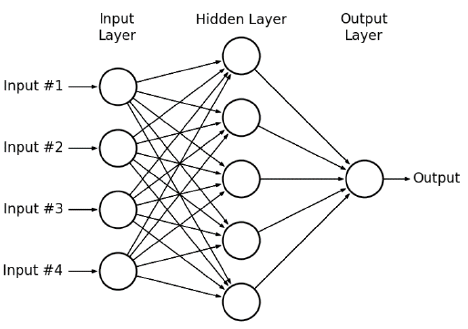
\includegraphics[width=0.8\linewidth]{A-hypothetical-example-of-Multilayer-Perceptron-Network}
		\caption{Architecture of Multi-layered perceptron}
		\label{fig:MLP_1}
	\end{figure}  
 	It contains one output neuron, but the number of output neurons can easily be extended to be more than one. 
 	
 	\subsection{\textbf{Activation function}} The activation function of a neuron maps the output of a neuron based on the total input that the neuron has received ( called the induced field of the neuron). The activation function can be linear or non-linear in nature. \\ Mathematically, the output $ y $ of $ j^{th} $ neuron is related to it's activation function $ \phi(.) $ as:  \begin{align}
 	\label{eq:MLP_act_func}
	y_{j} = \phi(\sum_{i=0}^{n}w_{ij}x_{i})
 	\end{align}
 	
 	Where: \begin{align*}
 	w_{ij} &= weight \: of \: j^{th} \: neuron \: connecting \: i^{th} \: input \\
 	x_{i} &= i^{th} \: input \: in \: the \: input \: vector
 	\end{align*}
 	
 	Different activation functions are used in practice. Some of the typical ones include: \\
 	\subsubsection{Linear} Here, $$ \phi(x) = x $$. This is used typically in the input layer, and also in output layer for regression tasks. \\
 	
 	\subsubsection{Sigmoid} Here $$ \phi(x) = \frac{1}{1-e^{-\lambda x}} $$. This lies in range $ [0, 1] $. It is typically used in hidden layers in pattern classification tasks. \\
 	
 	\subsubsection{Hyperbolic Tangent} Here $$ \phi(x) = \tanh(\lambda x) $$. It permits negative output in contrast to sigmoid, and is used in cases where a negative output is expected. This is the one we used in out hidden layers as activation function.\\ \\ 
 	
 	The characteristics of different activation functions are shown in figure \ref{fig:activationfunctions}
\begin{figure}[h]
	\centering
	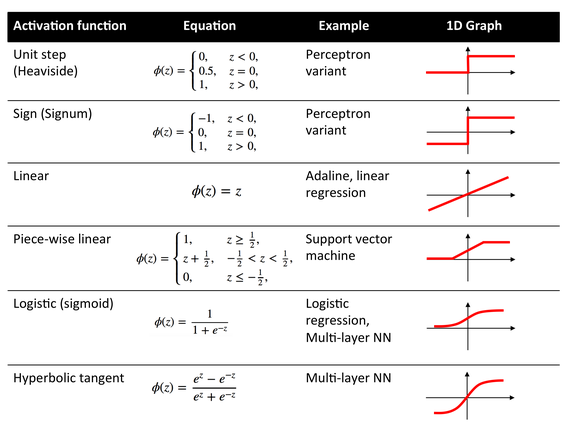
\includegraphics[width=0.8\linewidth]{activation_functions}
	\caption{A small list of activation functions}
	\label{fig:activationfunctions}
\end{figure}

\subsection{\textbf{Learning}} Learning refers to the process, where the neural network learns to update it's weights based on given input pattern set. Three distinct learning procedures exist: \\ 

\subsubsection{\textit{Supervised Learning}} Here, the network is presented with a pattern set $ \tau\{X^{k}, D^{k}\} $, with input vectors $ X^{k} $ and corresponding target output vectors $ D^{k} $, where $ k $ is the iteration index. The network learns the functional mapping $ f(X^{k}) = D^{k} $ through the learning algorithm. The learning process proceeds as follows: \\ \begin{enumerate}
	\item The network is initialized with random weights, and the input pattern $ X_{k} $ is presented to the network, and the corresponding output $ y_{k} $ is noted. \\
	\item The mean-squared error $ e_{k} = \frac{1}{2}\sum_{k}(D_{k}-y_{k})^{2} $ is calculated from target vector $ D_{k} $. \\
	\item The weights are updated using backpropagation algorithm, by propagating the error backwards. The details of the algorithm can be found in 
	% ref to backpropagation 
	and is not discussed in detail here. \\
\end{enumerate}

\subsubsection{Reinforcement Learning} Here, the network is given a set of input vectors, and a reward, based on the action taken by the network. The network tries to maximize the reward, through learning algorithm, typical one being Q-learning. \\
\subsubsection{Unsupervised Learning} Unsupervised learning forces the network to learn from input data alone. Typically, the network is trained to cluster the inputs into different sets, by a distance measure. \\

MLPs are universal function approximators as showed by Cybenko's theorem, so they can be used to create mathematical models by regression analysis. As classification is a particular case of regression when the response variable is categorical, MLPs make good classifier algorithms.
\subsection{Training a MLP in Matlab} Matlab R2017a provides a built-in feedforwardnet class, which can be used to create our simple two layer MLP network. The default activation functions are \textbf{Hyperbolic Tangent} in hidden layer, and \textbf{Linear} in output layer. The sample implementation we used is shown  below: 
\begin{minted}[
frame=lines,
framesep=2mm,
baselinestretch=1.2,
linenos
]{matlab}
% feedforwardnet is the net class
% 50 is the number of hidden layer neurons
net = feedforwardnet(50); 		
net.divideParam.trainRatio = 0.7;		
net.divideParam.valRatio = 0.3;

%Train for 50 epochs
net.trainParam.epochs = 50;				
net.trainParam.max_fail = 50;
net.trainParam.min_grad = 0;

% X is input vector; D is target vector
net = train(net, X', D');
\end{minted}
 
 After the training is over, the simulink block is formed by gensim command as follows 
 \begin{minted}{matlab}	
 gensim(net)
 \end{minted}
 
 The Simulink block can now be used for testing in simulink models.
\section{Elman networks} 
%TODO: By Asim
Asim's part
\section{System Identification} System identification is the process of developing a mathematical model of a dynamic system based on the input and output data from the actual process. This means it is possible to sample the input and output signals of a system and using this data generate a mathematical model. An important stage in control system design is the development of a mathematical model of the system to be controlled. In order to develop a controller, it must be possible to analyse the system to be controlled and this is done using a mathematical model. Another advantage of system identification is evident if the process is changed or modified. System identification allows the real system to be altered without having to calculate the dynamical equations and model the parameters again. \\ \\

System identification is concerned with developing models. The inverted pendulum system is a non-linear process. To adequately
model it, non-linear methods using neural networks must be used.
\subsection{System Identification Procedure}
Basically system identification is achieved by adjusting the parameters of the model until the
model output is similar to the output of the real system. The basic procedure is modelled in figure \ref{fig:Sys_Identification_block}
\begin{figure}[h!]
\centering
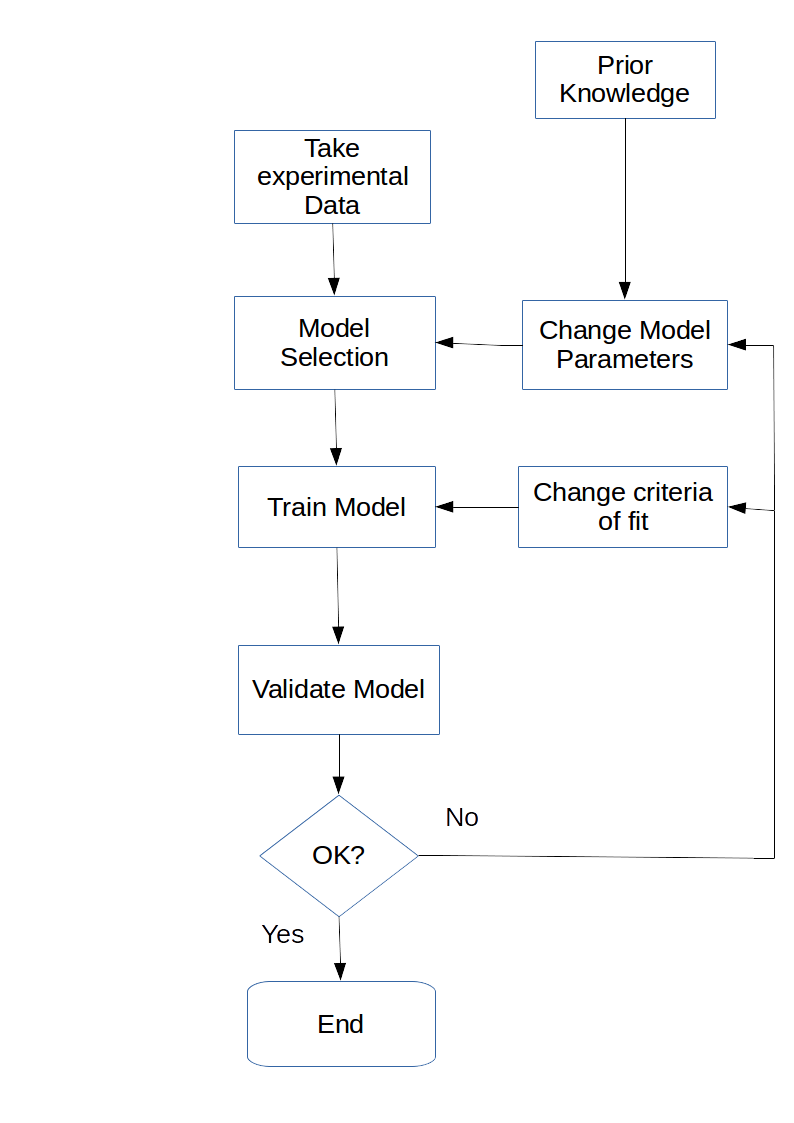
\includegraphics[width=0.7\linewidth]{Sys_Identification_block}
\caption{System Identification Procedure}
\label{fig:Sys_Identification_block}
\end{figure}

The main steps in system identification are: \\ \begin{enumerate}
	\item The first step is to generate some experimental input/output data from the process we
	are trying to model. In the case of the inverted pendulum system this would be the
	input force on the cart and the output pendulum angle. The data is split into 70\% training set and 15\% validation set.  
	\item The next step is to choose a model structure to use. We shall use multi-layer perceptrons, and elman networks. The parameters are initialized to random values.
	\item Next, the model is trained in a supervised fashion from the input/output data generated using backpropagation algorithm.
	\item The network is validated against a validation set. If validation accuracy is good enough, then the modeel is accepted, else, the model parameters are changed, and the training is performed again.
\end{enumerate}

\subsection{Non-Linear Identification of the Process with neural networks} This section discusses the different methods of identifying the pendulum process using neural
networks. The most common method of neural network identification is called forward
modelling ( shown in figure \ref{fig:forward_modelling}). During training both the process and ANN receive the same input,
the outputs from the ANN and process are compared, this error signal is used to update the
weights in the ANN. This is an example of supervised learning- the teacher (pendulum
system) provides target values for the learner (the neural network). 
\begin{figure}[h!]
\centering
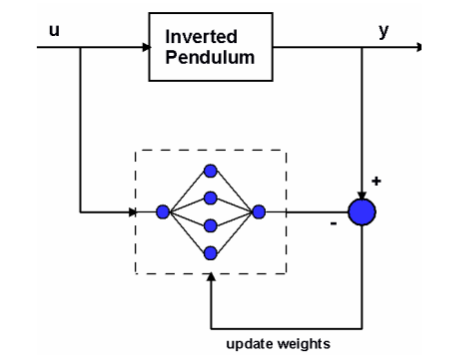
\includegraphics[width=0.7\linewidth]{forward_modelling}
\caption{Forward modelling procedure ( Taken from Callinan etal)}
\label{fig:forward_modelling}
\end{figure}

\subsubsection{Generation of training data} The Simulink model of Pendulum+ Feedback Linearized controller is excited from a sine-wave, to which band-limited noise has been added. This forms the input vector $ X $. The Plant produces 4 state vectors: Position$ x $, Velocity$ x^{.} $, Pendulum angle $ \theta $, Pendulum angular velocity $ \theta^{.} $. In the single output identification case, we consider only the angle $ \theta $ as the output vector. The Simulink model of the process is shown below:
%TODO: Add simulink block os feedback linearized controller

Thus, we get our training sample $ \tau = {X, D} $. Thsi will be used in training of the neural nets for system identification.

\subsubsection{Identification with MLP} 
%TODO
\subsubsection{Identification with Elman nets}
%TODO
\subsubsection{Multi-output Identification}
%TODO
\section{Conclusion}
	

\end{document}